%%%%%%%%%%%%%%%%%%%%%%%%%%%%%%%%%%%%%%%%%%%%%%%%%%%%%%%%%%%%%%%%%%%%%%%%%%%%%%%%
\section{Selecting Curated Workflows}
{   
	\usebackgroundtemplate{
		\vbox to \paperheight{\vfil\hbox to \paperwidth{\hfil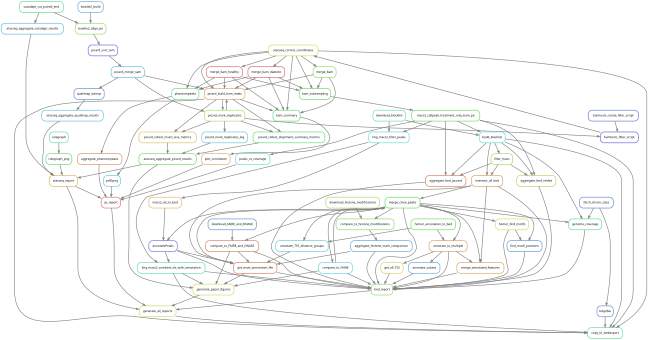
\includegraphics[height=.7\paperheight]{example_dags/rulegraph_complex.png}\hfil}\vfil}
	}
	\frame{
		\frametitle{Selecting Workflows}
		\begin{mdframed}[tikzsetting={draw=white,fill=white,fill opacity=0.8,
				line width=0pt},backgroundcolor=none,leftmargin=0,
			rightmargin=150,innertopmargin=4pt,roundcorner=10pt]
			\tableofcontents[currentsection,sections={1-4},hideothersubsections]
		\end{mdframed}
	}
}


%%%%%%%%%%%%%%%%%%%%%%%%%%%%%%%%%%%%%%%%%%%%%%%%%%%%%%%%%%%%%%%%%%%%%%%%%%%%%%%%
\begin{frame}
  \frametitle{What is this about?}
   \begin{question}[Questions]
   	 \begin{itemize}
       \item How do I get a workflow for a given scientific problem?
       \item How do I run such an arbitrary workflow?
     \end{itemize}
   \end{question} 
   \begin{docs}[Objectives]
   	  \begin{enumerate}
                      \item Introducing the workflow catalogue?
                      \item Learning the difference between ``curation'' (what some people think) and ``curation'' (what really works)?
      \end{enumerate}
    \end{docs}
\end{frame}  

\subsection{The Snakemake Workflow Catalogue}

%%%%%%%%%%%%%%%%%%%%%%%%%%%%%%%%%%%%%%%%%%%%%%%%%%%%%%%%%%%%%%%%%%%%%%%%%%%%%%%
\begin{frame}
 \frametitle{Selecting and Downloading from the Workflow Catalogue}
 You can find the \Snakemake{} worfkflow catalogue, \lhref{https://snakemake.github.io/snakemake-workflow-catalog/?rules=true}{here}. It makes a difference between workflows which meet best-practice criteria - and those which do not.\newline
 \begin{columns}
   \begin{column}{0.5\textwidth}
     You can download and run any workflow. \Snakemake's portability features ensure it will work everywhere.\pause
     \begin{warning}
     	Except, you most likely cannot, because of a missing cluster configuration and some missing features.
     \end{warning}
   \end{column}
   \begin{column}{0.5\textwidth}
     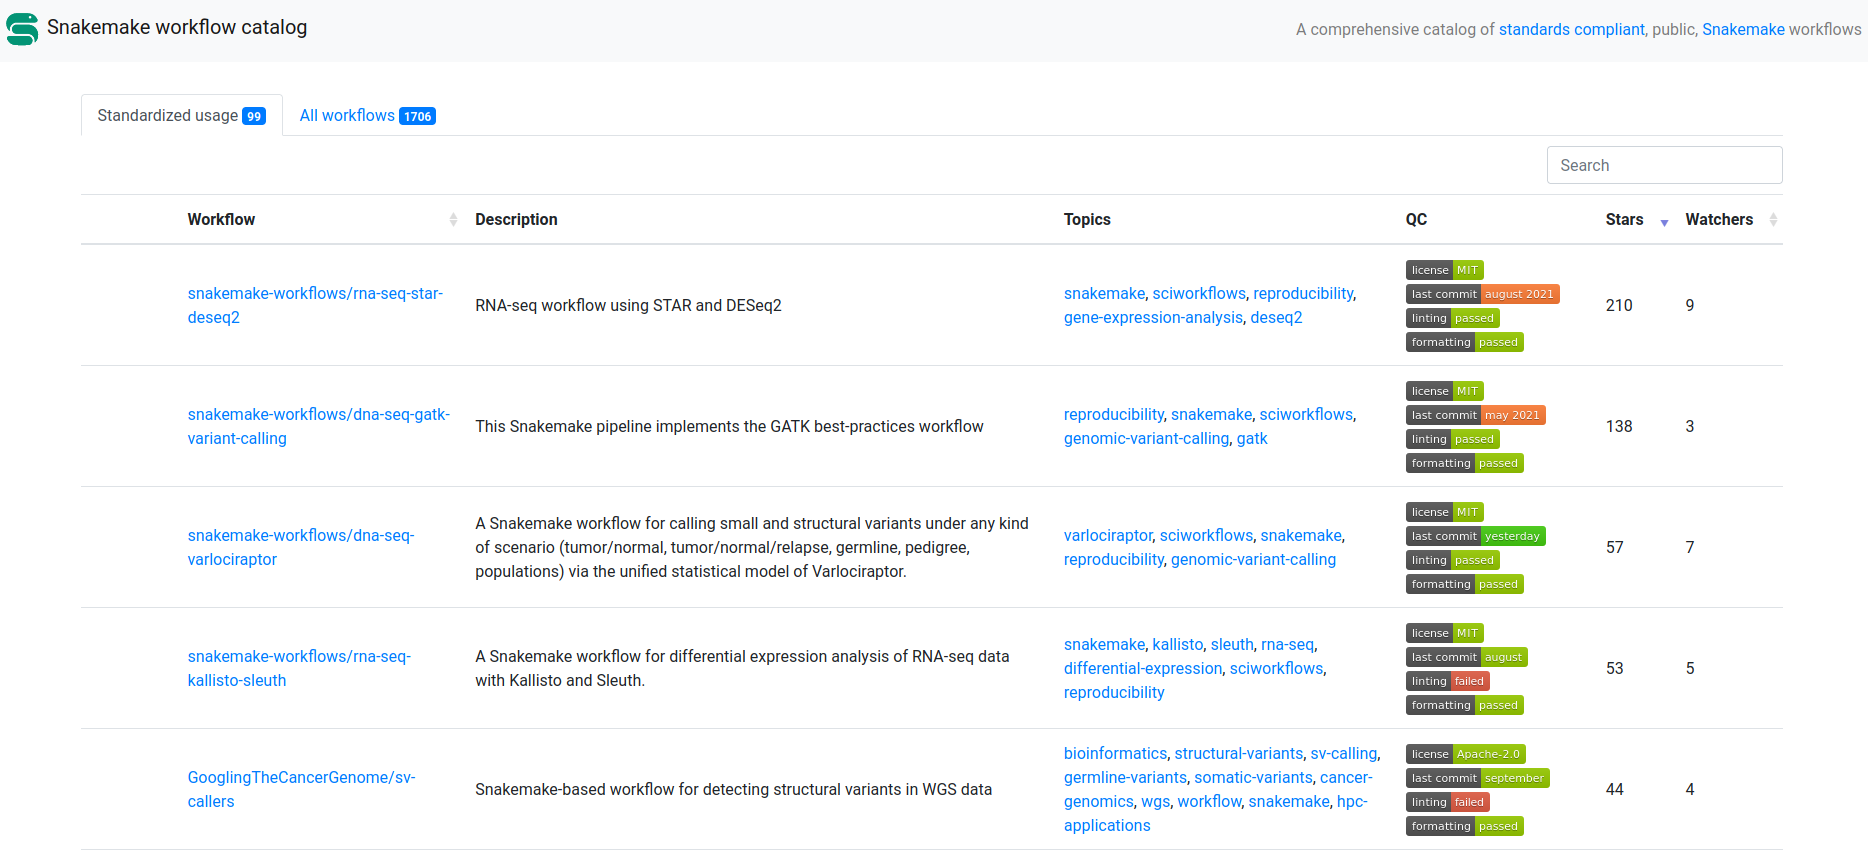
\includegraphics[width=\textwidth]{Snakemake/Snakemake_Workflow_Catalog.png}
   \end{column}
 \end{columns}
\end{frame}

%%%%%%%%%%%%%%%%%%%%%%%%%%%%%%%%%%%%%%%%%%%%%%%%%%%%%%%%%%%%%%%%%%%%%%%%%%%%%%%
\begin{frame}
  \frametitle{Searching \emph{your} Workflow}
   \begin{columns}
  	\begin{column}{0.5\textwidth}
  		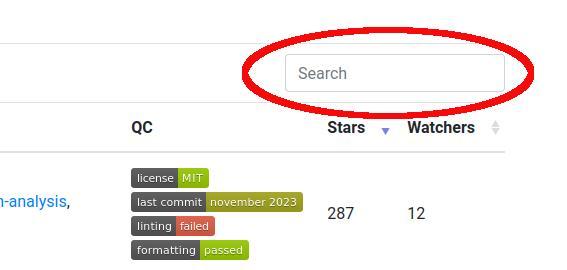
\includegraphics[width=\textwidth]{Snakemake/Searching_Workflows_in_Catalog.png}
  	\end{column}
  	\begin{column}{0.5\textwidth}
  		You can look for 
  		\begin{itemize}
  		  \item topical keywords
  		  \item software
  		\end{itemize}
  	\end{column}
  \end{columns}
\end{frame}

%%%%%%%%%%%%%%%%%%%%%%%%%%%%%%%%%%%%%%%%%%%%%%%%%%%%%%%%%%%%%%%%%%%%%%%%%%%%%%%
\begin{frame}
	\frametitle{Workflows Compliance}
	\begin{question}[Noted this?]
	  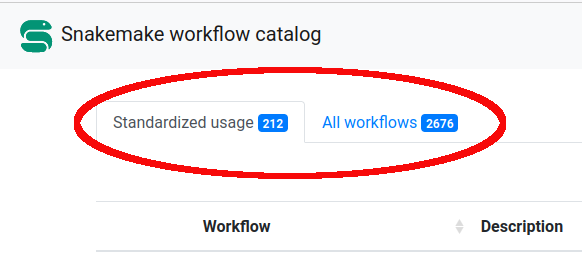
\includegraphics[width=0.8\textwidth]{Snakemake/Snakemake_Workflow_Catalog_Categories.png}
	\end{question}
\end{frame}

%%%%%%%%%%%%%%%%%%%%%%%%%%%%%%%%%%%%%%%%%%%%%%%%%%%%%%%%%%%%%%%%%%%%%%%%%%%%%%%%
\begin{frame}[fragile]
  \frametitle{Deployment}
  Select (=click on) any desired workflow. There are three alternatives:
  \begin{enumerate}[<+->]
   \item a workflow offers a release - in which case you can download and unpack it
   \item all workflows offers a ``\altverb{git clone}'' hint
   \item or you use the \altverb{snakedeploy} to get everything you need.
  \end{enumerate}
\end{frame}

%%%%%%%%%%%%%%%%%%%%%%%%%%%%%%%%%%%%%%%%%%%%%%%%%%%%%%%%%%%%%%%%%%%%%%%%%%%%%%%%
\begin{frame}[fragile]
	\frametitle{Deployment II - Creating an Environment Fork}
	Instead of creating environment from scratch we can clone one:
	\begin{lstlisting}[language=Bash, style=Shell]
$ mamba create -n <name of new env> --clone snakemake
    \end{lstlisting}
    This should clone the \altverb{snakemake} environment with all necessary tools!
    \pause
    \begin{task}
    	Pick one workflow from the catalogue, create a new environment with a corresponding name, e.\,g. \altverb{rna-seq-star}. Activate it. Then, install \altverb{snakedeploy}.
    \end{task}
    \pause
\end{frame}

%%%%%%%%%%%%%%%%%%%%%%%%%%%%%%%%%%%%%%%%%%%%%%%%%%%%%%%%%%%%%%%%%%%%%%%%%%%%%%%%
\begin{frame}[fragile]
	\frametitle{Deployment III - Let's do it!}
	Follow step 2 of a selected workflow usage instructions:
	\begin{center}
	    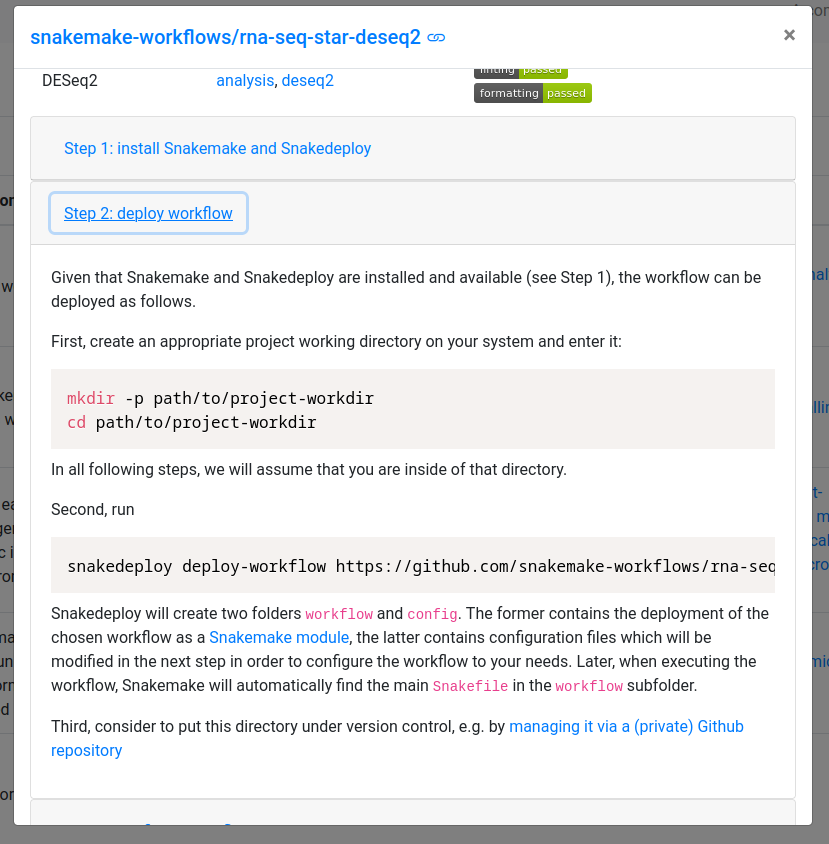
\includegraphics[width=0.6\textwidth]{Snakemake/deploy_workflow}
    \end{center}
\end{frame}

%%%%%%%%%%%%%%%%%%%%%%%%%%%%%%%%%%%%%%%%%%%%%%%%%%%%%%%%%%%%%%%%%%%%%%%%%%%%%%%%
\begin{frame}[fragile]
  \frametitle{Running Workflows on Cluster (or other environment)}
  Most likely a specific workflow never has been testing on \emph{your} computer before. It is almost ensured it will run on arbitrary servers, but clusters are a different story. \newline
  So
  \begin{itemize}[<+->]
   \item try to parameterize your workflow as learned
   \item if it gives issues and you know how to correct it, ``fork'' the worklow and create a pull request
   \item if you cannot fix it, create a bug report
  \end{itemize}
\end{frame}

%%%%%%%%%%%%%%%%%%%%%%%%%%%%%%%%%%%%%%%%%%%%%%%%%%%%%%%%%%%%%%%%%%%%%%%%%%%%%%%%
\begin{frame}
  \frametitle{\Interlude{Learn git!}}
  If you do not know what ``fork'' and ``pull request'' means, learn git!
  \begin{itemize}[<+->]
   \item there are courses
   \item and lots of online material
   \item and books
  \end{itemize}
  \pause
  \begin{warning}
  	Knowing git is essential in data analysis!
  \end{warning}
\end{frame}


